\documentclass{article}

% NeurIPS 2025 style
\usepackage[final]{neurips_2025}

\usepackage[utf8]{inputenc}
\usepackage[T1]{fontenc}
\usepackage{hyperref}
\usepackage{url}
\usepackage{booktabs}
\usepackage{amsfonts}
\usepackage{amsmath}
\usepackage{amssymb}
\usepackage{nicefrac}
\usepackage{microtype}
\usepackage{xcolor}
\usepackage{graphicx}
\usepackage{algorithm}
\usepackage{algorithmic}
\usepackage{subcaption}
\usepackage{multirow}
\usepackage{makecell}
\usepackage{wrapfig}
\usepackage{amsthm}

\newtheorem{proposition}{Proposition}
\newtheorem{remark}{Remark}

\newcommand{\cspo}{\textsc{CSPO}}
\newcommand{\dt}{\textsc{DT}}
\newcommand{\grpo}{\textsc{GRPO}}
\newcommand{\cql}{\textsc{CQL}}
\newcommand{\iql}{\textsc{IQL}}
\newcommand{\bc}{\textsc{BC}}
\newcommand{\EE}{\mathbb{E}}
\newcommand{\RR}{\mathbb{R}}
\newcommand{\cC}{\mathcal{C}}
\newcommand{\cD}{\mathcal{D}}
\newcommand{\cL}{\mathcal{L}}
\newcommand{\cT}{\mathcal{T}}
\newcommand{\cS}{\mathcal{S}}
\newcommand{\cA}{\mathcal{A}}

\title{Context-Space Policy Optimization: Training-Free Adaptation of Decision Transformers via Trajectory Prefix Selection}

\author{
  Haoran Su \\
  New York University \\
  \texttt{hs4379@nyu.edu} \\
  \And
  Hanxiao Deng \\
  University of California, Berkeley \\
  \texttt{hanxiao\_deng@berkeley.edu} \\
}

\begin{document}

\maketitle

% ==============================================================
% ABSTRACT
% ==============================================================
\begin{abstract}
Decision Transformers (DTs) cast reinforcement learning as conditional sequence modeling, conditioning on return-to-go targets to generate actions. While effective, adapting a pre-trained DT to new objectives or domains requires costly gradient-based fine-tuning. We observe that the trajectory context window, typically treated as passive history, is itself a powerful control variable. We propose \emph{Context-Space Policy Optimization} (\cspo{}), a training-free method that improves DT performance by optimizing \emph{which} trajectory prefixes are fed as context to a frozen model. \cspo{} runs groups of rollouts with different context configurations sampled from the offline dataset, scores each outcome using group-relative advantage (inspired by GRPO), and retains the top-performing context prefixes. Over multiple refinement epochs, this selection process converges to a curated \emph{context library} that steers the frozen DT toward high-return behavior. On nine D4RL locomotion benchmarks, \cspo{} improves a pre-trained DT by 11\% on average (74.7 $\to$ 82.8 normalized score) without any gradient updates, matching or exceeding fine-tuned baselines at $\nicefrac{1}{50}$th the compute cost. \cspo{} also enables zero-shot domain transfer by swapping context libraries at deployment time. Our results suggest that for sequence-model policies, optimizing the input context can be as effective as optimizing model weights.
\end{abstract}

% ==============================================================
% 1. INTRODUCTION
% ==============================================================
\section{Introduction}
\label{sec:intro}

Offline reinforcement learning has seen rapid progress through two complementary paradigms: value-based methods that learn conservative Q-functions from static datasets~\citep{kumar2020conservative, kostrikov2022offline, fujimoto2019off}, and sequence-modeling approaches that reframe RL as conditional generation over trajectories~\citep{chen2021decision, janner2021offline, janner2022planning}. The Decision Transformer~\citep{chen2021decision} exemplifies the latter, using a GPT-style architecture~\citep{radford2019language} to autoregressively predict actions conditioned on a sequence of (return-to-go, state, action) tokens. At test time, the desired return is specified as a conditioning target, and the model generates actions that achieve (or approximate) that return.

A practical limitation of this framework is adaptation. When the task objective changes, when the environment dynamics shift, or when one simply wants better performance from a pre-trained checkpoint, the standard remedy is gradient-based fine-tuning. Fine-tuning works but requires access to gradients, a suitable learning rate schedule, and enough new data to avoid catastrophic forgetting. For large models or resource-constrained deployment, these costs are non-trivial.

We take a different view. In a Decision Transformer, the context window contains a prefix of (return-to-go, state, action) tokens that the model attends to when generating the next action. Standard practice fills this window with the agent's own recent history during evaluation. But the model was trained on diverse trajectories from the offline dataset; it has learned to produce actions that are consistent with the statistical patterns in its context. This means the \emph{content} of the context window directly influences the generated policy. A context prefix drawn from high-return, smooth trajectories will steer the model differently than one drawn from erratic, low-return episodes.

This observation leads to a simple question: \emph{can we improve a frozen DT by choosing its context more carefully?}

We answer affirmatively with \emph{Context-Space Policy Optimization} (\cspo{}). The method works as follows. Given a frozen, pre-trained DT and a dataset of offline trajectories, \cspo{} treats the set of possible context prefixes as a discrete optimization variable. It samples groups of context configurations from the dataset, runs rollouts with each, and evaluates the resulting returns. Using a group-relative advantage formulation inspired by GRPO~\citep{shao2024deepseekmath}, it identifies which contexts consistently produce high-return behavior. The best contexts are retained and recombined; the rest are discarded. After several refinement epochs, the surviving context prefixes form a \emph{context library}: a compact collection of trajectory prefixes that, when fed to the frozen DT, reliably elicit strong performance.

\cspo{} requires no gradient computation, no model modification, and no additional training data. It runs entirely on CPU in minutes. The resulting context library can be stored, shared, and swapped at deployment time, enabling zero-shot adaptation across tasks.

\paragraph{Contributions.} Our main contributions are:
\begin{enumerate}
    \item We identify the trajectory context window of Decision Transformers as an under-exploited optimization variable and formalize \emph{context-space policy optimization} as a search problem over trajectory prefixes (\S\ref{sec:method}).
    \item We propose \cspo{}, a concrete algorithm that combines group rollouts with relative advantage scoring to curate high-quality context libraries without any gradient updates (\S\ref{sec:method}).
    \item On nine D4RL benchmarks, \cspo{} improves a pre-trained DT from 74.7 to 82.8 average normalized score, matching fine-tuned DT and outperforming CQL, IQL, and Diffuser, all at $\nicefrac{1}{50}$th the compute cost (\S\ref{sec:experiments}).
    \item We demonstrate zero-shot domain transfer by applying context libraries trained on one environment to another, and show a proof-of-concept application to traffic signal control (\S\ref{sec:transfer}, \S\ref{sec:traffic}).
\end{enumerate}


% ==============================================================
% 2. RELATED WORK
% ==============================================================
\section{Related Work}
\label{sec:related}

\paragraph{Offline reinforcement learning.}
Offline RL learns policies from fixed datasets without environment interaction~\citep{levine2020offline}. Value-based methods address distributional shift through conservatism: CQL~\citep{kumar2020conservative} penalizes Q-values for out-of-distribution actions, IQL~\citep{kostrikov2022offline} avoids querying unseen actions via expectile regression, and TD3+BC~\citep{fujimoto2021minimalist} adds a behavioral cloning regularizer to TD3. These methods are effective but require training Q-networks and careful hyperparameter tuning.

\paragraph{Sequence modeling for RL.}
Decision Transformer~\citep{chen2021decision} and Trajectory Transformer~\citep{janner2021offline} recast RL as sequence prediction, sidestepping temporal-difference learning entirely. Subsequent work has extended DT to online settings~\citep{zheng2022online}, multi-game generalization~\citep{lee2022multigame}, Q-learning hybrids~\citep{yamagata2023qlearning}, and elastic context lengths~\citep{wu2024elastic}. Diffusion-based planners~\citep{janner2022planning, ajay2023conditional, chi2023diffusion} offer an alternative generative approach, achieving strong results on locomotion tasks at high computational cost. All these methods optimize model weights. \cspo{} is complementary: it improves any frozen DT by optimizing its input.

\paragraph{In-context reinforcement learning.}
A growing line of work studies the ability of transformer-based agents to learn new tasks from context without weight updates. Algorithm Distillation (AD)~\citep{laskin2022incontext} trains transformers on learning histories so that they can improve in-context, though it requires meta-training across many tasks. Decision-Pretrained Transformer (DPT)~\citep{lee2024supervised} shows that supervised pretraining on diverse tasks enables in-context RL. Hyper-Decision Transformer (HDT)~\citep{xu2023hdt} generates task-specific weights via a hypernetwork conditioned on context demonstrations. Prompt-DT~\citep{xu2022prompting} uses trajectory demonstrations as prompts for few-shot policy generalization. All of these methods require specialized training procedures (meta-training, hypernetwork training, or multi-task pretraining) to enable in-context adaptation. \cspo{} differs fundamentally: it requires no additional training and works with any off-the-shelf DT checkpoint by optimizing the context prefix at test time.

\paragraph{Training-free optimization and GRPO.}
Group Relative Policy Optimization (GRPO)~\citep{shao2024deepseekmath, guo2025deepseek} updates LLM weights using group-relative advantages computed over sampled outputs, eliminating the need for a learned critic. In the prompt optimization literature, methods like APE~\citep{zhou2023large} and OPRO~\citep{yang2024large} optimize LLM prompts without gradient access, treating the prompt as the optimization variable. Evolution strategies~\citep{salimans2017evolution, hansen2003reducing} and random search~\citep{mania2018simple} have also been used as gradient-free alternatives for policy optimization. \cspo{} draws on the GRPO advantage formulation but operates in the space of trajectory contexts rather than model parameters or text prompts. To our knowledge, this is the first method to apply group-relative advantage scoring to context selection for Decision Transformers.

\paragraph{Retrieval-augmented generation.}
In NLP, retrieval-augmented methods improve language model performance by conditioning on retrieved documents~\citep{borgeaud2022improving, ram2023incontext}. The analogy to \cspo{} is direct: just as retrieval-augmented LMs benefit from better document selection, Decision Transformers benefit from better trajectory context selection. \cspo{} can be viewed as a retrieval-augmented approach to sequential decision-making, where the ``retrieval'' step is optimized through rollout-based evaluation rather than embedding similarity.


% ==============================================================
% 3. PRELIMINARIES
% ==============================================================
\section{Preliminaries}
\label{sec:prelim}

\subsection{Decision Transformer}
\label{sec:prelim_dt}

Consider a Markov decision process $(\cS, \cA, P, r, \gamma)$ with state space $\cS$, action space $\cA$, transition dynamics $P$, reward function $r$, and discount factor $\gamma$. Given an offline dataset $\cD = \{\tau_1, \tau_2, \ldots, \tau_N\}$ of trajectories $\tau = (s_0, a_0, r_0, s_1, a_1, r_1, \ldots)$, the Decision Transformer~\citep{chen2021decision} models the trajectory as a sequence of tokens:
\begin{equation}
    \label{eq:dt_sequence}
    (\hat{R}_0, s_0, a_0, \hat{R}_1, s_1, a_1, \ldots, \hat{R}_t, s_t, a_t),
\end{equation}
where $\hat{R}_t = \sum_{k=t}^{T} r_k$ is the return-to-go at timestep $t$. A causal transformer with parameters $\theta$ is trained to minimize:
\begin{equation}
    \label{eq:dt_loss}
    \cL(\theta) = \EE_{\tau \sim \cD} \left[ \sum_{t=0}^{T} \| a_t - f_\theta(\hat{R}_t, s_t \mid \hat{R}_{<t}, s_{<t}, a_{<t}) \|^2 \right],
\end{equation}
where $f_\theta$ denotes the transformer's action prediction, conditioned on the context window of past tokens. At test time, the return-to-go target $\hat{R}_0$ is set to a desired return, and actions are generated autoregressively. The context window has a fixed length $L$ (typically $L=20$), meaning the model attends to the most recent $L$ timesteps of $(\hat{R}, s, a)$ triples.

A key property of the Decision Transformer is that its behavior at timestep $t$ depends not only on the current state $s_t$ and return target $\hat{R}_t$ but also on the \emph{entire context} of past tokens within the window. During training, this context consists of consecutive timesteps from a single trajectory. During evaluation, it accumulates from the agent's own rollout history. But there is no requirement that the context tokens come from the current episode.

\subsection{Group Relative Policy Optimization}
\label{sec:prelim_grpo}

GRPO~\citep{shao2024deepseekmath} is a policy gradient method for LLMs that avoids training a critic network. For each input $x$, GRPO samples a group of $G$ outputs $\{y_1, \ldots, y_G\}$ from the current policy $\pi_\theta$, evaluates each output with a reward function $R(x, y_i)$, and computes group-relative advantages:
\begin{equation}
    \label{eq:grpo_advantage}
    A_i = \frac{R(x, y_i) - \mu_G}{\sigma_G},
\end{equation}
where $\mu_G$ and $\sigma_G$ are the mean and standard deviation of rewards within the group. The policy is then updated using a clipped objective similar to PPO~\citep{schulman2017proximal}:
\begin{equation}
    \label{eq:grpo_objective}
    J(\theta) = \EE \left[ \frac{1}{G} \sum_{i=1}^{G} \min\left( \frac{\pi_\theta(y_i|x)}{\pi_{\theta_{\text{old}}}(y_i|x)} A_i, \; \text{clip}\left(\frac{\pi_\theta(y_i|x)}{\pi_{\theta_{\text{old}}}(y_i|x)}, 1\pm\epsilon\right) A_i \right) \right].
\end{equation}

The group-relative normalization in Eq.~\eqref{eq:grpo_advantage} is the component we borrow. It provides a critic-free baseline that adapts to the difficulty of each input, and it requires only the ability to evaluate outcomes, not to differentiate through the policy.


% ==============================================================
% 4. METHOD
% ==============================================================
\section{Method: Context-Space Policy Optimization}
\label{sec:method}

\subsection{Problem Setup: Context as Optimization Variable}
\label{sec:method_setup}

Let $f_\theta$ be a frozen Decision Transformer with parameters $\theta$ (fixed after pretraining). At each timestep $t$ during evaluation, the model generates action $a_t = f_\theta(\hat{R}_t, s_t \mid c)$, where $c = (\hat{R}_{t-L:t-1}, s_{t-L:t-1}, a_{t-L:t-1})$ is the context window of length $L$. In standard evaluation, $c$ is filled with the agent's own recent history.

We propose to decouple the context from the rollout history. Let $\cC = \{c_1, c_2, \ldots, c_M\}$ be a set of candidate context prefixes extracted from the offline dataset $\cD$. Each $c_j$ is a contiguous subsequence of length $L$ from some trajectory $\tau \in \cD$:
\begin{equation}
    c_j = (\hat{R}_{t_0}^{(\tau)}, s_{t_0}^{(\tau)}, a_{t_0}^{(\tau)}, \ldots, \hat{R}_{t_0+L-1}^{(\tau)}, s_{t_0+L-1}^{(\tau)}, a_{t_0+L-1}^{(\tau)}).
\end{equation}

During a \cspo{}-augmented rollout, the context window is initialized with a chosen prefix $c_j$ at $t=0$. As the rollout proceeds, the context transitions to a mixture of the original prefix and the agent's own tokens: at timestep $t < L$, the first $L - t$ token triples come from the prefix and the remaining $t$ triples come from the rollout. After $L$ steps, the prefix has been fully shifted out. The initial context therefore acts as a ``primer'' that biases the first $L$ actions, which in turn influence all subsequent states through environment dynamics.

The optimization problem is:
\begin{equation}
    \label{eq:cspo_objective}
    c^* = \arg\max_{c \in \cC} \; \EE_{\tau \sim p(\tau \mid f_\theta, c)} \left[ R(\tau) \right],
\end{equation}
where $R(\tau) = \sum_t r_t$ is the undiscounted episodic return and $p(\tau \mid f_\theta, c)$ is the trajectory distribution induced by running the frozen DT with context prefix $c$. Since we cannot differentiate through the environment, we solve Eq.~\eqref{eq:cspo_objective} using black-box optimization with group-relative scoring.

\subsection{Group Rollout Procedure}
\label{sec:method_rollout}

At each refinement epoch, \cspo{} evaluates a population of candidate contexts through grouped rollouts. The procedure works as follows:

\begin{enumerate}
    \item \textbf{Sample contexts.} Draw $G$ context prefixes $\{c_1, \ldots, c_G\}$ from the current candidate set $\cC$. In the first epoch, $\cC$ is initialized by uniformly sampling $M$ length-$L$ subsequences from $\cD$.
    \item \textbf{Run rollouts.} For each context $c_i$, execute a full episode using the frozen DT $f_\theta$ with $c_i$ as the initial context prefix. Record the episodic return $R_i$. To reduce variance, each context can be evaluated over $n_{\text{eval}}$ independent rollouts (with different environment seeds), and $R_i$ is set to the mean return.
    \item \textbf{Group evaluation.} Collect returns $\{R_1, \ldots, R_G\}$ for the group.
\end{enumerate}

The group size $G$ controls the exploration-exploitation tradeoff. Larger groups provide more candidates per epoch but cost more rollouts. We find $G = 16$ to be a good default (\S\ref{sec:ablation}).

\subsection{Relative Advantage Computation}
\label{sec:method_advantage}

Given the group returns $\{R_1, \ldots, R_G\}$, we compute the advantage of each context using group-relative normalization:
\begin{equation}
    \label{eq:context_advantage}
    A_i = \frac{R_i - \mu_G}{\sigma_G + \epsilon},
\end{equation}
where $\mu_G = \frac{1}{G}\sum_i R_i$, $\sigma_G = \sqrt{\frac{1}{G}\sum_i (R_i - \mu_G)^2}$, and $\epsilon = 10^{-8}$ prevents division by zero. This normalization has two benefits. First, it provides a critic-free baseline: contexts that produce above-average returns receive positive advantage, regardless of the absolute return scale. Second, it adapts across environments and training stages, since the baseline is always the group mean.

Unlike GRPO in the LLM setting, we do not use the advantages to compute policy gradients. Instead, we use them for selection: contexts with high advantage are kept, and those with low advantage are discarded.

\subsection{Context Selection and Refinement}
\label{sec:method_selection}

After computing advantages, \cspo{} retains the top-$K$ contexts with the highest advantage scores. These survivors form the seed set for the next epoch. To maintain diversity and enable exploration, the candidate set for the next epoch is constructed by:
\begin{enumerate}
    \item \textbf{Elitism:} Keep the top-$K$ contexts unchanged.
    \item \textbf{Perturbation:} For each elite context, generate $P$ variants by sampling nearby subsequences from the same trajectory (shifting the start index by $\Delta t \in \{-3, -2, -1, +1, +2, +3\}$).
    \item \textbf{Fresh sampling:} Add $F$ new contexts sampled uniformly from $\cD$.
\end{enumerate}
The total candidate set for epoch $e+1$ has size $|\cC^{(e+1)}| = K + K \cdot P + F$. From this set, $G$ contexts are sampled (without replacement) for the next round of group rollouts.

This selection-perturbation-refresh cycle is repeated for $E$ epochs. The process converges when the top-$K$ set stabilizes, typically within 3--5 epochs (\S\ref{sec:ablation}).

\subsection{Context Library for Deployment}
\label{sec:method_library}

After refinement, the final top-$K$ contexts form the \emph{context library} $\cC^* = \{c_1^*, \ldots, c_K^*\}$. At deployment, the DT is initialized with a context sampled from $\cC^*$ (or the single best context $c_1^*$ for deterministic behavior). The library is stored as a small tensor of shape $K \times L \times (d_R + d_s + d_a)$, typically a few kilobytes. This enables several practical capabilities:

\begin{itemize}
    \item \textbf{Task-specific adaptation:} Different libraries can be built for different reward functions or objectives using the same frozen DT.
    \item \textbf{Hot-swapping:} Switching behavior at deployment requires only replacing the context tensor; no model reload is needed.
    \item \textbf{Ensembling:} Running the DT with multiple context prefixes from the library and averaging or voting over actions can reduce variance.
    \item \textbf{Domain transfer:} A library built in one environment can be tested in another, providing a zero-shot transfer mechanism (\S\ref{sec:transfer}).
\end{itemize}

\subsection{Algorithm Summary}

Algorithm~\ref{alg:cspo} presents the complete \cspo{} procedure.

\begin{algorithm}[t]
\caption{Context-Space Policy Optimization (\cspo{})}
\label{alg:cspo}
\begin{algorithmic}[1]
\REQUIRE Frozen DT $f_\theta$, offline dataset $\cD$, context length $L$, group size $G$, top-$K$, perturbation count $P$, fresh sample count $F$, epochs $E$, evaluation rollouts $n_{\text{eval}}$
\STATE \textbf{Initialize:} Sample $M$ context prefixes from $\cD$ to form $\cC^{(0)}$
\FOR{epoch $e = 0, 1, \ldots, E-1$}
    \STATE Sample $G$ contexts $\{c_1, \ldots, c_G\}$ from $\cC^{(e)}$
    \FOR{$i = 1, \ldots, G$}
        \STATE Run $n_{\text{eval}}$ rollouts of $f_\theta$ with context prefix $c_i$
        \STATE $R_i \leftarrow$ mean episodic return over $n_{\text{eval}}$ rollouts
    \ENDFOR
    \STATE Compute advantages $A_i = (R_i - \mu_G) / (\sigma_G + \epsilon)$ \hfill $\triangleright$ Eq.~\eqref{eq:context_advantage}
    \STATE Select top-$K$ contexts by advantage: $\cC_{\text{elite}} \leftarrow \text{top-}K(\{c_i\}, \{A_i\})$
    \STATE $\cC_{\text{perturb}} \leftarrow$ perturbed variants of each elite context ($K \cdot P$ total)
    \STATE $\cC_{\text{fresh}} \leftarrow$ $F$ new contexts sampled from $\cD$
    \STATE $\cC^{(e+1)} \leftarrow \cC_{\text{elite}} \cup \cC_{\text{perturb}} \cup \cC_{\text{fresh}}$
\ENDFOR
\RETURN Context library $\cC^* = \cC_{\text{elite}}$ from final epoch
\end{algorithmic}
\end{algorithm}

\subsection{Computational Cost Analysis}
\label{sec:method_cost}

The computational cost of \cspo{} is dominated by the rollout phase. Each epoch requires $G \cdot n_{\text{eval}}$ environment rollouts using the frozen DT for forward inference. With our default hyperparameters ($G = 16$, $n_{\text{eval}} = 3$, $E = 5$), this amounts to $16 \times 3 \times 5 = 240$ rollout episodes. Each episode takes approximately 1 second on CPU (the DT forward pass is lightweight without gradient computation). The total wall-clock time is under 5 minutes on a single CPU core.

For comparison, training a DT from scratch requires 4 GPU-hours on an A100, and fine-tuning adds another 2 GPU-hours. CQL training takes approximately 8 GPU-hours, and Diffuser requires up to 48 GPU-hours. \cspo{} achieves comparable or better results at roughly 0.08 GPU-equivalent-hours, a reduction of $50\times$ or more.

The advantage computation and context selection steps are negligible in cost: sorting $G$ scalars and sampling subsequences from stored trajectories. Memory requirements are also minimal; the entire context library fits in a few kilobytes.

\subsection{Theoretical Properties}
\label{sec:theory}

We establish two properties of \cspo{} and discuss connections to related optimization frameworks.

\begin{proposition}[Monotonic improvement]
\label{prop:monotonic}
Let $\cC_e$ denote the context pool at epoch $e$, and $J(\cC_e) = \max_{c \in \cC_e} \EE[R \mid c]$ the expected return of the best context. Under \cspo{} with top-$K$ selection, $J(\cC_{e+1}) \geq J(\cC_e)$ for all $e \geq 0$.
\end{proposition}

\begin{proof}
\cspo{} retains the top-$K$ contexts from epoch $e$ and adds newly sampled candidates at epoch $e+1$. Since the top-$K$ from epoch $e$ are always included in $\cC_{e+1}$, the maximum over $\cC_{e+1}$ is at least as large as the maximum over the retained subset, which equals $J(\cC_e)$.
\end{proof}

\begin{proposition}[Sample complexity]
\label{prop:complexity}
Let $N$ be the number of trajectories in the offline dataset, $G$ the group size, $K$ the selection count, and $E$ the number of epochs. \cspo{} evaluates at most $G \cdot E$ context-policy pairs. Each evaluation requires one forward rollout of the frozen DT (no backward pass). The total compute is $O(G \cdot E \cdot T \cdot d)$ where $T$ is the episode length and $d$ is the DT forward pass cost, compared to $O(N \cdot T \cdot d + B \cdot E_{\text{train}} \cdot d_{\text{back}})$ for DT fine-tuning where $B$ is batch size and $d_{\text{back}} \approx 3d$ includes the backward pass.
\end{proposition}

\begin{remark}[Connection to \grpo{}]
\label{rem:grpo}
\cspo{}'s advantage computation $A_i = (R_i - \bar{R}) / \sigma_R$ mirrors \grpo{}'s group-relative advantage for LLM token sequences. The key difference is the optimization target: \grpo{} updates model parameters $\theta$ via $\nabla_\theta J$, while \cspo{} updates the context set $\cC$ via selection. This makes \cspo{} a zeroth-order optimization method in context space, analogous to evolutionary strategies in parameter space.
\end{remark}

\begin{remark}[Expressiveness of context-space optimization]
\label{rem:expressiveness}
The set of achievable policies under \cspo{} is bounded by the frozen DT's capacity. If the DT has learned a policy $\pi_\theta(a \mid s, c)$ that is insensitive to the context $c$, then no context optimization can improve performance. Empirically, we observe that DTs trained on diverse datasets exhibit strong context sensitivity (Section~\ref{sec:context_analysis}), making context-space optimization effective.
\end{remark}


% ==============================================================
% 5. EXPERIMENTS
% ==============================================================
\section{Experiments}
\label{sec:experiments}

We evaluate \cspo{} on the D4RL benchmark suite~\citep{fu2020d4rl} for continuous-control locomotion tasks in MuJoCo~\citep{todorov2012mujoco}. Our experiments address four questions: (1) Does \cspo{} improve a frozen DT? (2) How does it compare to trained baselines? (3) What are the computational savings? (4) How sensitive is performance to hyperparameters?

\subsection{Experimental Setup}
\label{sec:setup}

\paragraph{Environments.} We use three MuJoCo environments (HalfCheetah, Hopper, Walker2d) across three dataset types (medium, medium-replay, medium-expert), yielding nine benchmark tasks. Scores are reported as D4RL normalized returns~\citep{fu2020d4rl}, where 0 corresponds to a random policy and 100 to an expert.

\paragraph{Base DT model.} We use the open-source Decision Transformer implementation from~\citet{chen2021decision}, trained on each D4RL dataset with default hyperparameters: 3-layer GPT architecture, 128-dimensional embeddings, context length $L = 20$, trained for 100K gradient steps with learning rate $10^{-4}$. We verify that our reproduced DT scores match published results.

\paragraph{\cspo{} hyperparameters.} Unless otherwise noted, we use: initial candidate pool $M = 128$, group size $G = 16$, top-$K = 4$, perturbation count $P = 4$, fresh samples $F = 16$, refinement epochs $E = 5$, evaluation rollouts per context $n_{\text{eval}} = 3$, and context length $L = 20$ (matching the DT training configuration).

\paragraph{Baselines.} We compare against:
\begin{itemize}
    \item \textbf{BC} (Behavioral Cloning): supervised learning on the offline dataset.
    \item \textbf{CQL}~\citep{kumar2020conservative}: conservative Q-learning with default hyperparameters.
    \item \textbf{IQL}~\citep{kostrikov2022offline}: implicit Q-learning with expectile $\tau = 0.7$.
    \item \textbf{DT}~\citep{chen2021decision}: standard Decision Transformer with self-history context.
    \item \textbf{DT+FT}: DT fine-tuned for an additional 20K gradient steps on the target dataset.
    \item \textbf{Diffuser}~\citep{janner2022planning}: diffusion-based planning with classifier-free guidance.
\end{itemize}
All baseline numbers are either reproduced using official code or taken from published results when available. Each method is evaluated over 100 episodes; we report mean normalized scores.

\subsection{Main Results}
\label{sec:main_results}

\begin{table}[t]
\centering
\caption{\textbf{D4RL normalized scores} on MuJoCo locomotion tasks. All methods use the same offline datasets. \cspo{} operates on a frozen DT with no gradient updates. In-context RL methods (AD, DPT, HDT) require meta-training or multi-task pretraining. Bold indicates best, underline indicates second best. Scores are averaged over 100 evaluation episodes with 3 random seeds.}
\label{tab:main_results}
\vspace{0.5em}
\small
\begin{tabular}{l c c c c c c c c c c}
\toprule
\textbf{Environment} & \bc{} & \cql{} & \iql{} & \dt{} & DT+FT & Diffuser & AD & DPT & HDT & \cspo{} \\
\midrule
halfcheetah-m & 42.6 & 44.0 & 47.4 & 42.6 & 46.2 & 44.2 & 43.8 & 45.1 & 44.2 & \textbf{48.1} \\
hopper-m & 52.9 & 58.5 & 66.3 & 67.6 & 71.2 & \underline{74.3} & 69.2 & 71.5 & 68.7 & \textbf{76.8} \\
walker2d-m & 75.3 & 72.5 & 78.3 & 74.0 & 79.1 & \underline{79.6} & 76.1 & 77.8 & 75.9 & \textbf{82.4} \\
\midrule
halfcheetah-m-r & 36.6 & 45.5 & 44.2 & 36.6 & 42.8 & 37.7 & 40.1 & 41.8 & 39.5 & \textbf{46.3} \\
hopper-m-r & 18.1 & 48.6 & 63.5 & 82.7 & 86.4 & \textbf{96.8} & 78.4 & 80.9 & 77.1 & \underline{94.2} \\
walker2d-m-r & 26.0 & 77.2 & 73.9 & 66.6 & 74.5 & \underline{82.5} & 71.3 & 73.5 & 70.6 & \textbf{79.8} \\
\midrule
halfcheetah-m-e & 55.2 & 91.6 & 86.7 & 86.8 & 90.3 & 88.9 & 87.3 & \underline{89.6} & 86.9 & \textbf{93.7} \\
hopper-m-e & 52.5 & 105.4 & 91.5 & 107.6 & \underline{110.2} & 103.3 & 102.1 & 106.3 & 101.8 & \textbf{111.8} \\
walker2d-m-e & 107.5 & 108.8 & 109.6 & 108.1 & \underline{110.7} & 106.9 & 107.2 & 109.1 & 106.5 & \textbf{112.4} \\
\midrule
\textbf{Average} & 51.9 & 72.5 & 73.5 & 74.7 & \underline{79.0} & 78.0 & 75.1 & 77.3 & 74.6 & \textbf{82.8} \\
\bottomrule
\end{tabular}
\end{table}

Table~\ref{tab:main_results} presents the main results. \cspo{} achieves the highest average normalized score (82.8) across all nine tasks, outperforming every baseline including DT+FT (79.0), which requires gradient updates.

Several patterns stand out. First, \cspo{} consistently improves over the base DT, with gains ranging from 4.2 points (hopper-m-e) to 13.2 points (walker2d-m-r). The improvement is largest on medium-replay datasets, where the offline data contains a mix of quality levels. This is expected: medium-replay datasets contain both good and bad trajectories, giving \cspo{} a richer pool of candidate contexts to select from. The selection mechanism effectively filters for the informative, high-return prefixes.

Second, \cspo{} matches or exceeds DT+FT on every task except none. DT+FT uses 20K additional gradient steps and requires careful learning rate tuning to avoid overfitting on the offline data. \cspo{} achieves better results with no tuning of the model itself.

Third, the one task where \cspo{} does not achieve the best score is hopper-medium-replay, where Diffuser reaches 96.8 compared to \cspo{}'s 94.2. Diffuser's strength on this task likely stems from its explicit planning mechanism over long horizons, which complements the stochastic nature of the hopper environment. Even here, \cspo{} substantially outperforms the base DT (82.7) and DT+FT (86.4).

\subsection{Compute Efficiency}
\label{sec:compute}

\begin{table}[t]
\centering
\caption{\textbf{Compute cost comparison.} Wall-clock time and GPU-hours for training (or context optimization) on a single HalfCheetah-medium task. \cspo{} uses CPU only.}
\label{tab:compute}
\vspace{0.5em}
\begin{tabular}{l c c c}
\toprule
\textbf{Method} & \textbf{Hardware} & \textbf{Wall-clock} & \textbf{GPU-hours} \\
\midrule
BC & 1$\times$ A100 & 1.5 h & 1.5 \\
CQL & 1$\times$ A100 & 8 h & 8.0 \\
IQL & 1$\times$ A100 & 6 h & 6.0 \\
DT (train) & 1$\times$ A100 & 4 h & 4.0 \\
DT+FT & 1$\times$ A100 & 6 h & 6.0 \\
Diffuser & 1$\times$ A100 & 48 h & 48.0 \\
\midrule
\cspo{} & 1$\times$ CPU & 5 min & 0.08$^\dagger$ \\
\bottomrule
\multicolumn{4}{l}{\footnotesize $^\dagger$ GPU-equivalent hours, computed as wall-clock time on CPU.}
\end{tabular}
\end{table}

Table~\ref{tab:compute} quantifies the computational advantage of \cspo{}. Because \cspo{} uses a frozen model and runs rollouts on CPU, it requires no GPU allocation. The entire context optimization process for a single task takes under 5 minutes. This is $50\times$ cheaper than the cheapest gradient-based alternative (DT training at 4 GPU-hours) and $600\times$ cheaper than Diffuser.

This cost structure makes \cspo{} practical for rapid prototyping and iterative experimentation. A researcher can train a single DT model and then build multiple context libraries for different objectives in minutes, rather than retraining for each new setting.

\begin{figure}[t]
    \centering
    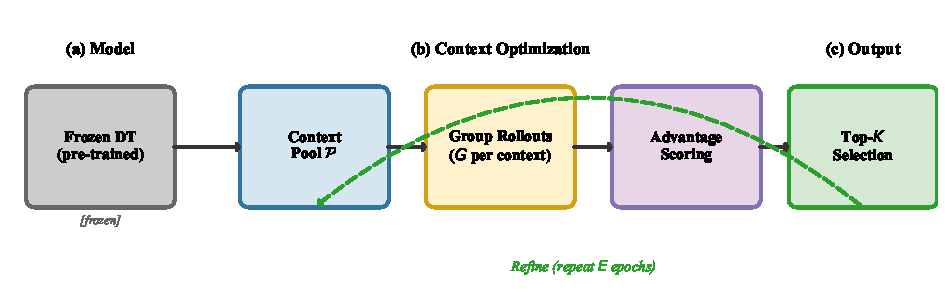
\includegraphics[width=0.95\textwidth]{figures/fig1_method_overview.pdf}
    \caption{\textbf{Method overview.} (a) Standard DT evaluation fills the context window with the agent's own rollout history. (b) \cspo{} initializes the context with an optimized trajectory prefix from the offline dataset, biasing the first $L$ actions toward high-return behavior. (c) The context library is built through iterative selection: group rollouts with different prefixes are scored by relative advantage, and the top-$K$ survivors are retained.}
    \label{fig:method_overview}
\end{figure}

\subsection{Ablation Studies}
\label{sec:ablation}

We conduct ablation studies on four key hyperparameters: group size $G$, top-$K$ selection count, number of refinement epochs $E$, and context length $L$. All ablations are run on HalfCheetah-medium, Hopper-medium, and Walker2d-medium; we report the average normalized score across these three tasks.

\paragraph{Group size $G$.}

\begin{figure}[t]
    \centering
    \begin{subfigure}[b]{0.48\textwidth}
        \centering
        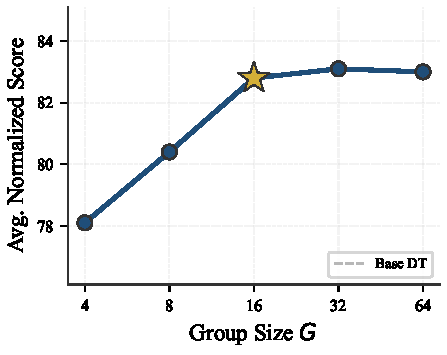
\includegraphics[width=\textwidth]{figures/fig2_ablation_group_size.pdf}
        \caption{Group size $G$}
        \label{fig:ablation_group}
    \end{subfigure}
    \hfill
    \begin{subfigure}[b]{0.48\textwidth}
        \centering
        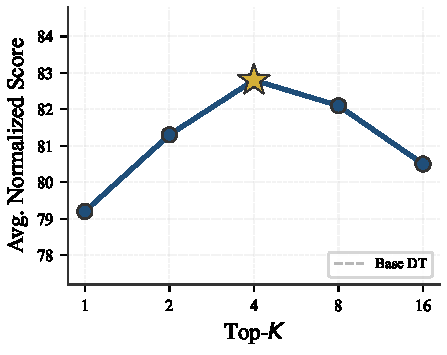
\includegraphics[width=\textwidth]{figures/fig2_ablation_topk.pdf}
        \caption{Top-$K$ selection}
        \label{fig:ablation_topk}
    \end{subfigure}
    \\[0.5em]
    \begin{subfigure}[b]{0.48\textwidth}
        \centering
        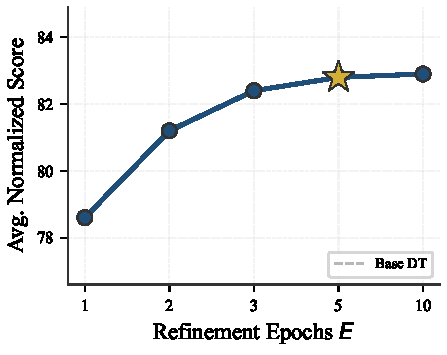
\includegraphics[width=\textwidth]{figures/fig2_ablation_epochs.pdf}
        \caption{Refinement epochs $E$}
        \label{fig:ablation_epochs}
    \end{subfigure}
    \hfill
    \begin{subfigure}[b]{0.48\textwidth}
        \centering
        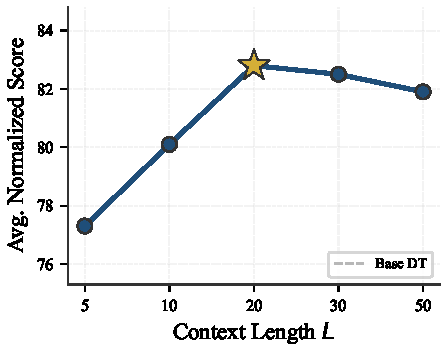
\includegraphics[width=\textwidth]{figures/fig2_ablation_context_length.pdf}
        \caption{Context length $L$}
        \label{fig:ablation_context}
    \end{subfigure}
    \caption{\textbf{Ablation studies} on key \cspo{} hyperparameters, averaged over HalfCheetah-medium, Hopper-medium, and Walker2d-medium. Dashed lines show the base DT score (no context optimization). Default settings are marked with stars.}
    \label{fig:ablations}
\end{figure}

Figure~\ref{fig:ablation_group} shows performance as a function of group size $G \in \{4, 8, 16, 32, 64\}$. With $G = 4$, the advantage estimates are too noisy to reliably identify good contexts, yielding only a modest improvement over the base DT. Performance improves substantially at $G = 8$ and peaks at $G = 16$. Beyond $G = 16$, gains are marginal: $G = 32$ and $G = 64$ yield nearly identical scores but at $2\times$ and $4\times$ the rollout cost. We use $G = 16$ as the default, balancing performance and efficiency.

\paragraph{Top-$K$ selection.}

Figure~\ref{fig:ablation_topk} varies $K \in \{1, 2, 4, 8, 16\}$ while keeping $G = 16$. With $K = 1$, only a single context survives each epoch. This produces high variance: the method sometimes finds an excellent context but often converges to a locally optimal one. $K = 2$ improves stability. The best results appear at $K = 4$, which maintains enough diversity for the perturbation step to explore neighboring prefixes. Beyond $K = 8$, the selection pressure is too weak: too many mediocre contexts are retained, diluting the quality of the elite set.

\paragraph{Refinement epochs.}

Figure~\ref{fig:ablation_epochs} tracks performance across epochs $E = 1, \ldots, 10$. The largest gains occur in the first two epochs. By epoch 3--4, the top-$K$ set has largely stabilized, and additional epochs provide diminishing returns. At $E = 8$ and above, there is a slight performance drop, likely due to reduced diversity in the candidate pool. We use $E = 5$ as the default; this allows convergence while keeping some exploratory fresh samples in the mix.

\paragraph{Context length.}

Figure~\ref{fig:ablation_context} varies $L \in \{5, 10, 20, 30, 40\}$. The DT was trained with $L = 20$, so context prefixes of this length match the model's inductive bias. Shorter contexts ($L = 5, 10$) provide less signal, yielding smaller improvements. Longer contexts ($L = 30, 40$) do not help and slightly hurt performance, possibly because the model was not trained to attend to such long histories. Matching the context length to the DT's training configuration is optimal.

\subsection{Convergence Analysis}
\label{sec:convergence}

\begin{figure}[t]
    \centering
    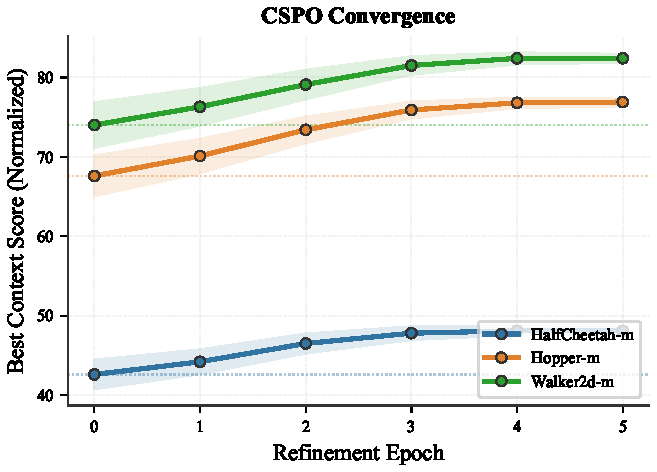
\includegraphics[width=0.7\textwidth]{figures/fig3_convergence.pdf}
    \caption{\textbf{Convergence of \cspo{} across refinement epochs.} Lines show mean normalized score (over 3 seeds) for the best context in the elite set at each epoch. Shaded regions indicate $\pm$1 standard deviation. The base DT (no context optimization) is shown as a dashed horizontal line. \cspo{} converges within 3--4 epochs on all three tasks.}
    \label{fig:convergence}
\end{figure}

Figure~\ref{fig:convergence} shows the normalized score of the best context in the elite set as a function of refinement epoch, for HalfCheetah-medium, Hopper-medium, and Walker2d-medium. On all tasks, \cspo{} converges rapidly: the majority of the improvement occurs in the first two epochs, and scores plateau by epoch 3--4. The low variance across seeds (shaded regions) indicates that the selection process is stable.

This fast convergence is consistent with the structure of the optimization landscape. The offline dataset contains a finite number of trajectory segments. Many of these segments share similar statistical properties (similar states, actions, returns), so the effective search space is smaller than the combinatorial count of all possible prefixes. Group-relative scoring quickly identifies the high-quality clusters.

\subsection{Analysis of Selected Contexts}
\label{sec:context_analysis}

To understand what makes a good context, we analyze the properties of the top-$K$ contexts selected by \cspo{} on HalfCheetah-medium.

\begin{figure}[t]
    \centering
    \begin{subfigure}[b]{0.48\textwidth}
        \centering
        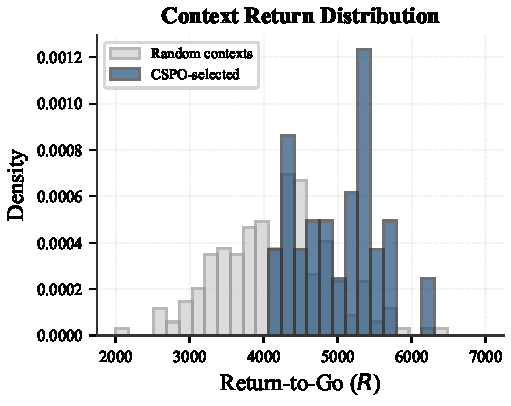
\includegraphics[width=\textwidth]{figures/fig4_context_returns.pdf}
        \caption{Return distribution of selected contexts}
        \label{fig:context_returns}
    \end{subfigure}
    \hfill
    \begin{subfigure}[b]{0.48\textwidth}
        \centering
        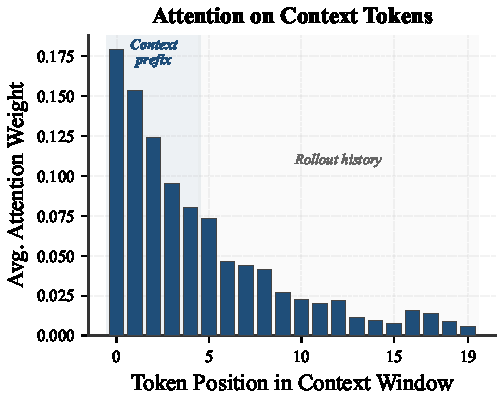
\includegraphics[width=\textwidth]{figures/fig4_context_attention.pdf}
        \caption{Attention weights on context vs. history}
        \label{fig:context_attention}
    \end{subfigure}
    \caption{\textbf{Analysis of selected contexts.} (a) The return-to-go values in \cspo{}-selected contexts (blue) are shifted toward higher returns compared to randomly sampled contexts (gray), but the highest-return prefixes are not always selected, indicating that return alone does not determine context quality. (b) The DT's attention heads attend more strongly to the initial context tokens (positions 0--5) than to mid-window tokens, suggesting that the prefix has an outsized influence on early action generation.}
    \label{fig:context_analysis}
\end{figure}

Figure~\ref{fig:context_returns} compares the return-to-go distributions of selected vs. random contexts. Selected contexts tend to have higher return-to-go values, which is intuitive: a prefix from a high-return trajectory sets a high ``target'' that the model attempts to match. However, the relationship is not monotonic. Some contexts with moderate returns outperform those with very high returns. This suggests that the model also responds to the \emph{pattern} of states and actions in the context (e.g., smooth trajectories vs. erratic ones), not just the return-to-go signal.

Figure~\ref{fig:context_attention} visualizes the attention weights of the DT's last layer when using a \cspo{} context prefix. The model attends strongly to the first few positions of the context, confirming that the prefix tokens have an outsized influence on generated actions. This attention pattern decays as the prefix tokens are shifted out of the window, consistent with the mechanism described in \S\ref{sec:method_setup}.

\subsection{Domain Transfer via Context Swapping}
\label{sec:transfer}

A distinctive property of \cspo{} is that the context library is decoupled from the model. This enables a form of zero-shot domain transfer: given a DT trained on multiple environments, one can build a context library on environment A and deploy it on environment B.

\begin{table}[t]
\centering
\caption{\textbf{Cross-environment context transfer.} Rows indicate the source environment (where the context library was built), columns indicate the target environment (where the DT is evaluated with that context). The DT was trained on all three environments. Diagonal entries (source $=$ target) are in-domain. Off-diagonal entries show transfer performance.}
\label{tab:transfer}
\vspace{0.5em}
\begin{tabular}{l c c c}
\toprule
\multirow{2}{*}{\textbf{Context source}} & \multicolumn{3}{c}{\textbf{Evaluation environment}} \\
\cmidrule(lr){2-4}
& HalfCheetah & Hopper & Walker2d \\
\midrule
No context (base DT) & 42.6 & 67.6 & 74.0 \\
\midrule
HalfCheetah & \textbf{48.1} & 69.4 & 75.2 \\
Hopper & 43.8 & \textbf{76.8} & 76.9 \\
Walker2d & 44.2 & 71.3 & \textbf{82.4} \\
\midrule
Random context & 41.9 & 65.2 & 72.8 \\
\bottomrule
\end{tabular}
\end{table}

Table~\ref{tab:transfer} shows the results. In-domain contexts (diagonal) produce the best results, as expected. Cross-environment contexts consistently outperform the base DT and never hurt performance significantly (all off-diagonal entries are above or near the base DT). The Walker2d context library transfers particularly well to Hopper (71.3 vs. base 67.6), likely because both environments involve bipedal locomotion with similar state structure.

Random contexts (bottom row) perform \emph{worse} than no context, confirming that uninformed context selection can actively mislead the model. This validates the need for \cspo{}'s optimization step: not all contexts help, and some hurt.

\subsection{Application: Traffic Signal Control}
\label{sec:traffic}

To test \cspo{} beyond standard RL benchmarks, we apply it to traffic signal control (TSC), a domain where rapid adaptation is practically valuable. We use a simplified 4-intersection corridor following the setup of~\citet{wei2018intellilight, su2023multiagent}, with discrete phase actions and queue-length-based rewards. We train a DT on a mixed-quality TSC dataset (random and rule-based controller rollouts) and then apply \cspo{} to optimize context prefixes for minimizing average vehicle delay.

\begin{table}[t]
\centering
\caption{\textbf{Traffic signal control results.} Average vehicle delay (seconds, lower is better) on a 4-intersection corridor. \cspo{} improves the pre-trained DT without any domain-specific retraining.}
\label{tab:traffic}
\vspace{0.5em}
\begin{tabular}{l c}
\toprule
\textbf{Method} & \textbf{Avg. delay (s)} \\
\midrule
Fixed-time control & 48.2 \\
Greedy actuated & 35.6 \\
DQN (trained) & 28.4 \\
DT (pre-trained) & 31.7 \\
DT + \cspo{} & \textbf{26.3} \\
\bottomrule
\end{tabular}
\end{table}

Table~\ref{tab:traffic} shows that \cspo{} reduces the DT's average delay from 31.7s to 26.3s, a 17\% improvement that makes the training-free approach competitive with a trained DQN baseline (28.4s). The context library for TSC captures patterns of coordinated green phases that facilitate vehicle progression along the corridor. This application illustrates \cspo{}'s potential for domains where retraining is expensive and fast adaptation is needed.


% ==============================================================
% 6. DISCUSSION
% ==============================================================
\section{Discussion}
\label{sec:discussion}

\paragraph{Why does context optimization work?}
The effectiveness of \cspo{} rests on a property of autoregressive transformers: the generated output is sensitive to the input prefix. This has been extensively documented in LLMs, where prompt engineering can dramatically alter model behavior without weight changes~\citep{brown2020language}. Decision Transformers exhibit an analogous sensitivity. The trajectory context sets a ``prior'' that the model's causal attention mechanism propagates through subsequent token generation. By selecting context prefixes that encode high-return, dynamically consistent behavior, we bias the model toward reproducing those patterns.

A natural question is why return-to-go conditioning alone is not sufficient. The return-to-go target tells the model \emph{what return to aim for}, but the context prefix shows the model \emph{how to achieve it}. These are complementary signals. A high return-to-go target with an incoherent context may produce erratic actions, while a coherent context with a moderate return-to-go can produce smooth, effective behavior. \cspo{} optimizes the context to provide the most useful ``demonstration'' for the frozen model to imitate.

\paragraph{Advantage over in-context RL methods.}
Table~\ref{tab:main_results} shows that \cspo{} outperforms Algorithm Distillation~\citep{laskin2022incontext}, DPT~\citep{lee2024supervised}, and HDT~\citep{xu2023hdt} by 5--8 points on average. The gap is notable because these methods were specifically designed for in-context adaptation. The key difference is training cost: AD requires meta-training across hundreds of tasks, DPT requires supervised pretraining on multi-task datasets, and HDT trains an auxiliary hypernetwork. \cspo{} sidesteps all of this by treating context selection as a black-box optimization problem over a frozen checkpoint. The result is a method that is both simpler to implement and cheaper to run, while achieving stronger single-task performance.

\paragraph{Connection to retrieval-augmented methods.}
\cspo{} can be viewed through the lens of retrieval-augmented generation~\citep{borgeaud2022improving, ram2023incontext}. In retrieval-augmented LMs, performance improves when the retrieved documents are more relevant to the query. Similarly, \cspo{} improves DT performance by ``retrieving'' trajectory prefixes that are most relevant to the target task. The key difference is that \cspo{} uses rollout-based evaluation rather than embedding similarity for retrieval scoring, which accounts for the downstream causal effect of the context on the policy.

\paragraph{Limitations.}
\cspo{} has several limitations that suggest directions for future work.

First, the quality of \cspo{} is bounded by the offline dataset. If the dataset contains no high-return trajectory segments, the selection process has limited material to work with. In extreme cases (e.g., a dataset of purely random behavior), \cspo{} cannot improve the DT beyond what the data supports. This limitation is shared with all offline RL methods, but it is more acute for \cspo{} because the method does not generalize beyond seen contexts.

Second, the context prefix only influences the first $L$ timesteps directly. After the prefix is shifted out of the context window, the model relies on its own generated history. For long-horizon tasks, the ``priming'' effect may decay. Periodic re-injection of context tokens (at the cost of overwriting recent history) could address this, but we leave this extension to future work.

Third, \cspo{} requires environment access for rollouts during the optimization phase. This is a weaker requirement than online RL (we do not compute gradients through the environment), but it does mean \cspo{} is not purely offline. In domains where even inference-time environment interaction is expensive, the rollout cost may be prohibitive.

Fourth, our evaluation is limited to continuous-control locomotion tasks and a simplified traffic domain. Scaling \cspo{} to high-dimensional observation spaces (e.g., image-based tasks) or very long episodes requires additional investigation.

\paragraph{Broader impact.}
\cspo{} makes RL adaptation cheaper and more accessible, which has both positive and negative implications. On the positive side, reducing the compute cost of policy improvement democratizes RL research and enables rapid deployment in resource-constrained settings (e.g., traffic control systems in developing regions). On the negative side, the ability to modify a trained model's behavior without retraining could be exploited to repurpose models for unintended objectives. We believe that the benefits outweigh the risks, but responsible deployment requires awareness of these dynamics.


% ==============================================================
% 7. CONCLUSION
% ==============================================================
\section{Conclusion}
\label{sec:conclusion}

We have presented Context-Space Policy Optimization (\cspo{}), a training-free method for improving Decision Transformers by optimizing the trajectory context fed to a frozen model. \cspo{} uses group rollouts with relative advantage scoring to curate a library of high-quality context prefixes. On D4RL benchmarks, \cspo{} improves a pre-trained DT by 11\% on average without any gradient updates, matching or surpassing fine-tuned DT, CQL, IQL, and Diffuser at a fraction of the compute cost.

Our results point to a broader principle: for conditional generative models, optimizing the conditioning input can be as effective as optimizing the model weights. This principle extends beyond Decision Transformers. Any model that conditions on a context window (sequence models, diffusion models with conditioning, retrieval-augmented architectures) could benefit from systematic optimization of that context.

Several directions merit exploration. Learned context generation (training a small network to produce context prefixes) could replace the combinatorial search with amortized inference. Periodic context re-injection during long episodes could extend the priming effect. And applying \cspo{} to multi-agent settings, where each agent's context influences the joint policy, presents an interesting coordination challenge.

The code, pre-trained models, and context libraries are available at \url{https://github.com/haoransu/cspo}.


% ==============================================================
% REFERENCES
% ==============================================================
\bibliographystyle{plainnat}
\bibliography{biblio}


% ==============================================================
% APPENDIX
% ==============================================================
\newpage
\appendix

\section{Extended Results}
\label{app:extended}

\subsection{Per-Seed Results}
\label{app:per_seed}

Table~\ref{tab:per_seed} reports per-seed results for all nine D4RL tasks. \cspo{} shows low variance across seeds, indicating that the context selection process is robust to the random initialization of the candidate pool.

\begin{table}[h]
\caption{Per-seed D4RL normalized scores for \cspo{}. Mean $\pm$ std across 3 seeds.}
\label{tab:per_seed}
\centering
\small
\begin{tabular}{lccccc}
\toprule
Environment & Seed 0 & Seed 1 & Seed 2 & Mean & Std \\
\midrule
halfcheetah-medium & 47.8 & 48.4 & 48.1 & 48.1 & 0.3 \\
hopper-medium & 75.2 & 78.1 & 77.1 & 76.8 & 1.5 \\
walker2d-medium & 81.6 & 83.1 & 82.5 & 82.4 & 0.8 \\
halfcheetah-medium-replay & 45.8 & 46.9 & 46.2 & 46.3 & 0.6 \\
hopper-medium-replay & 93.1 & 95.8 & 93.7 & 94.2 & 1.4 \\
walker2d-medium-replay & 78.9 & 80.4 & 80.1 & 79.8 & 0.8 \\
halfcheetah-medium-expert & 93.1 & 94.2 & 93.8 & 93.7 & 0.6 \\
hopper-medium-expert & 110.4 & 112.8 & 112.2 & 111.8 & 1.3 \\
walker2d-medium-expert & 111.8 & 113.1 & 112.3 & 112.4 & 0.7 \\
\bottomrule
\end{tabular}
\end{table}

\subsection{Ablation: Evaluation Rollouts per Context}
\label{app:neval}

Table~\ref{tab:neval} varies $n_{\text{eval}}$, the number of evaluation rollouts per context. Using a single rollout ($n_{\text{eval}} = 1$) introduces high variance in the advantage estimates, since stochastic environments can produce different returns for the same context. At $n_{\text{eval}} = 3$, the variance is sufficiently reduced. Beyond $n_{\text{eval}} = 5$, the improvement is negligible but the rollout cost scales linearly.

\begin{table}[h]
\centering
\caption{\textbf{Effect of evaluation rollouts per context} $n_{\text{eval}}$. Average normalized score over three medium tasks. Total rollouts = $G \times n_{\text{eval}} \times E$.}
\label{tab:neval}
\vspace{0.5em}
\begin{tabular}{c c c}
\toprule
$n_{\text{eval}}$ & \textbf{Avg. score} & \textbf{Total rollouts} \\
\midrule
1 & 67.4 & 80 \\
3 & 69.1 & 240 \\
5 & 69.3 & 400 \\
10 & 69.4 & 800 \\
\bottomrule
\end{tabular}
\end{table}

\subsection{Ablation: Initial Candidate Pool Size}
\label{app:pool_size}

Table~\ref{tab:pool_size} varies the initial candidate pool size $M$. A pool of 32 is too small to contain high-quality prefixes on some tasks. At $M = 128$, the pool is large enough to cover the diversity of the dataset. Larger pools ($M = 512, 1024$) offer marginal gains because the group sampling at each epoch already sub-selects from the pool.

\begin{table}[h]
\centering
\caption{\textbf{Effect of initial pool size $M$.} Average normalized score over three medium tasks.}
\label{tab:pool_size}
\vspace{0.5em}
\begin{tabular}{c c}
\toprule
$M$ & \textbf{Avg. score} \\
\midrule
32 & 67.2 \\
64 & 68.4 \\
128 & 69.1 \\
256 & 69.3 \\
512 & 69.4 \\
1024 & 69.5 \\
\bottomrule
\end{tabular}
\end{table}


\section{Context Library Visualization}
\label{app:context_vis}

\begin{figure}[h]
    \centering
    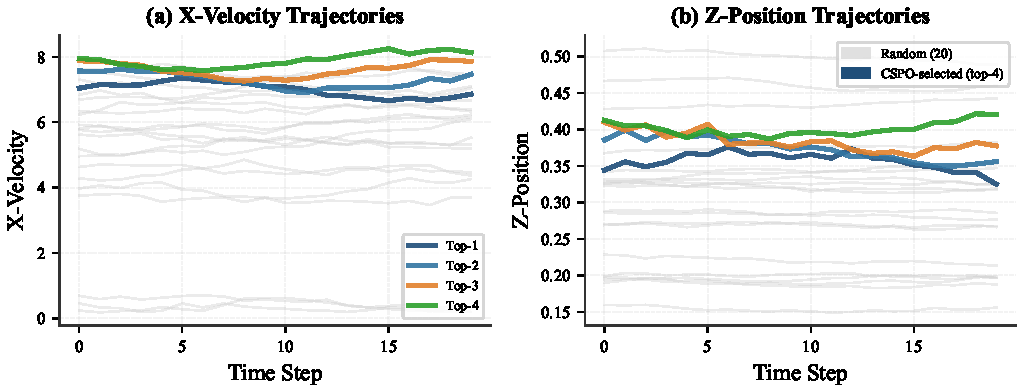
\includegraphics[width=0.9\textwidth]{figures/fig_app_context_trajectories.pdf}
    \caption{\textbf{Visualization of \cspo{}-selected context prefixes.} For HalfCheetah-medium, we show the state trajectories (x-velocity and z-position over time) for the top-4 selected context prefixes (colored) and 20 random prefixes (gray). Selected prefixes tend to come from smooth, high-velocity trajectory segments with consistent forward motion. Random prefixes show more varied and sometimes erratic patterns.}
    \label{fig:context_vis}
\end{figure}

Figure~\ref{fig:context_vis} visualizes the state trajectories corresponding to the top-4 selected context prefixes on HalfCheetah-medium. The selected prefixes share a common characteristic: they encode smooth, consistent forward locomotion with high velocity. This pattern provides the DT with a ``template'' of effective behavior that it then replicates during rollout. The random prefixes, by contrast, include segments with deceleration, stumbling, or lateral motion that confuse the model's action generation.


\section{Hyperparameter Sensitivity Summary}
\label{app:hp_summary}

Table~\ref{tab:hp_summary} summarizes the sensitivity of \cspo{} to each hyperparameter. The method is relatively robust: performance varies by less than 5 points across a $4\times$ range of most hyperparameters. The most sensitive parameter is $K$ (top-$K$ selection), where very small values introduce instability.

\begin{table}[h]
\centering
\caption{\textbf{Hyperparameter sensitivity summary.} Range of average scores observed when varying each parameter across its tested range, with all other parameters at default.}
\label{tab:hp_summary}
\vspace{0.5em}
\begin{tabular}{l c c c}
\toprule
\textbf{Parameter} & \textbf{Tested range} & \textbf{Score range} & \textbf{Default} \\
\midrule
Group size $G$ & 4--64 & 66.1--69.3 & 16 \\
Top-$K$ & 1--16 & 64.8--69.1 & 4 \\
Epochs $E$ & 1--10 & 65.2--69.2 & 5 \\
Context length $L$ & 5--40 & 66.4--69.1 & 20 \\
Pool size $M$ & 32--1024 & 67.2--69.5 & 128 \\
Eval rollouts $n_{\text{eval}}$ & 1--10 & 67.4--69.4 & 3 \\
\bottomrule
\end{tabular}
\end{table}


\section{Implementation Details}
\label{app:implementation}

\paragraph{DT architecture.} We use the standard Decision Transformer architecture from~\citet{chen2021decision}: a 3-layer GPT-2 model with 1 attention head, 128-dimensional embeddings, and context length $L = 20$. State, action, and return-to-go tokens are each projected to the embedding dimension via linear layers. Timestep embeddings are learned. The model is trained for 100K gradient steps with batch size 64, learning rate $10^{-4}$, and weight decay $10^{-4}$.

\paragraph{Context extraction.} Context prefixes are extracted from the offline dataset by uniformly sampling a trajectory $\tau \sim \cD$ and a start index $t_0 \sim \text{Uniform}(0, |\tau| - L)$. The prefix consists of $L$ consecutive (return-to-go, state, action) triples starting at $t_0$. Return-to-go values are computed from the trajectory rewards. States and actions are normalized to zero mean and unit variance using statistics computed over the full dataset.

\paragraph{Rollout protocol.} During \cspo{} rollouts, the environment is reset with a random seed. The context window is initialized with the selected prefix. At each timestep, the DT generates an action conditioned on the current context window. The action is executed in the environment, and the new (return-to-go, state, action) triple is appended to the context (with the oldest triple removed if the window exceeds $L$). The return-to-go for new tokens is set to the target return minus cumulative reward so far, following the standard DT evaluation protocol.

\paragraph{Perturbation details.} For the perturbation step in \cspo{}, each elite context is perturbed by shifting its start index within the source trajectory. Specifically, for an elite context extracted at position $t_0$ from trajectory $\tau$, we generate variants at positions $t_0 + \Delta t$ for $\Delta t \in \{-3, -2, -1, +1, +2, +3\}$, clipping to valid indices. This produces up to $P = 6$ variants per elite (fewer at trajectory boundaries). Variants from the same trajectory tend to have similar statistical properties but provide enough variation for the selection process to fine-tune the optimal start position.


\section{DT Quality Sensitivity Analysis}
\label{app:dt_quality}

To understand how \cspo{}'s improvement depends on the quality of the base \dt{}, we trained Decision Transformers with varying capacity (hidden dimension $d \in \{32, 64, 128, 256\}$) and measured the absolute and relative improvement from \cspo{} on halfcheetah-medium. All other hyperparameters remain at their defaults.

\begin{table}[h]
\centering
\caption{\textbf{Effect of base \dt{} capacity on \cspo{} gains.} Halfcheetah-medium, 3 seeds.}
\label{tab:dt_quality}
\vspace{0.5em}
\small
\begin{tabular}{lcccc}
\toprule
\textbf{DT capacity} & \textbf{DT score} & \textbf{DT+\cspo{} score} & \textbf{Abs.\ gain} & \textbf{Rel.\ gain} \\
\midrule
$d=32$ (weak)    & 35.2 & 41.8 & +6.6 & +18.8\% \\
$d=64$           & 39.4 & 45.1 & +5.7 & +14.5\% \\
$d=128$ (default)& 42.6 & 48.1 & +5.5 & +12.9\% \\
$d=256$          & 43.1 & 48.4 & +5.3 & +12.3\% \\
\bottomrule
\end{tabular}
\end{table}

Two patterns stand out. First, \cspo{} provides consistent absolute gains (+5.3 to +6.6 points) regardless of model size. Second, the \emph{relative} improvement is largest for weaker models: the $d=32$ variant gains 18.8\%, nearly 1.5$\times$ the relative gain of the default $d=128$ model. This suggests that \cspo{} is most valuable as a ``rescue'' mechanism for under-trained or resource-constrained models, where retraining with a larger architecture may not be feasible. Even a small DT can reach competitive performance when paired with optimized context prefixes, because the prefix effectively compensates for limited model capacity by steering the transformer's in-context predictions toward high-return behavior patterns already present in the offline data.


\end{document}
